%\documentclass{acm_proc_article-sp}

\documentclass{article}

\usepackage{mathpartir}
\usepackage{turnstile}
\usepackage{amssymb}
\usepackage{amsmath}
\usepackage{stmaryrd}
\usepackage{graphicx}
\usepackage{epsfig}
\usepackage{subfigure}
\usepackage{listings}
\usepackage{natbib}
\usepackage{verbatim}
\usepackage[utf8]{inputenc}
\usepackage[T1]{fontenc} 
\usepackage[hyphens]{url}
\lstset{language=ml}
\lstset{commentstyle=\textit}
\lstset{mathescape=true}
\lstset{backgroundcolor=,rulecolor=}
\lstset{frame=single}
\lstset{breaklines=true}
\lstset{basicstyle=\ttfamily}

\DeclareMathOperator{\wf}{wf}
\DeclareMathOperator{\acyclic}{acyclic}
\DeclareMathOperator{\Linear}{Linear}
\DeclareMathOperator{\NonLinear}{NonLinear}
\DeclareMathOperator{\range}{range}
\DeclareMathOperator{\FV}{FV}
\DeclareMathOperator{\LFV}{LFV}
\DeclareMathOperator{\rule-fun}{rule-fun}

\begin{document}

\title{Casanova: \\ a declarative language for safe games}

\author{
Giuseppe Maggiore \and Renzo Orsini \and Michele Bugliesi \\
\{maggiore,orsini,bugliesi\}@dais.unive.it
}

\date{}

\maketitle

\begin{abstract}
Games are extremely complex pieces of software which give life to animated virtual worlds. Games require complex algorithms, large worlds filled with many intelligent entities and high-quality graphics, and it all must run in real time.

Building general, high-performance frameworks capable of representing any virtual world has, until now, proven to be an elusive task; existing solutions either sacrifice performance (X3D browsers) or generality (game engines).

In this paper we present a model that formalizes our notion of a correct game. This model gives all the important properties that game developers struggle to maintain by hand, that is the strong normalization of the \texttt{tick} function, the independence from the order of the ticks of each entity, and the fact that all active entities of the game state must be ticked exactly once. We define the Casanova language around this model, with the aim of achieving the threefold objective of creating games that are correct, declarative (and thus simpler to write) and fast to run.

We will use a linear type system to enforce the uniqueness of our entities (to ensure exactly one tick for each) and to ensure that ticks do not have overlapping effects. We will impose certain restrictions on the state to avoid infinite loops in the update function (in the shape of cyclic references) and we will use a specialized type system to make sure that all the active coroutines of the game will always yield.
\end{abstract}

\begin{comment}
\category{D.1.1}{Programming Techniques}{Applicative (Functional) Programming} 
\category{D.2.2}{Soft\-ware Engineering}{Software Libraries}[Design Tools and Techniques]
\category{D.2.13}{Soft\-ware Engineering}{Reusable Software}[Domain engineering, Reusable libraries, Reuse models]
\category{D.3.3}{Programming Languages}{Language Constructs and Features}
\category{D.3.4}{Pro\-gramming Languages}{Processors}[Optimization, Run-time environments]
\category{H.5.1}{Information Systems}{Information Interfaces and Presentation}[Multimedia Information Systems]

\terms{Games,Performance,Languages}

\keywords{games, compilation}
\end{comment}

\section{Game Model}
\label{sec:game_model}
%%%%%%%%%%%%%%%%%%%%%%%%%%%%%%%%%%%%%%%%%%%%%%%%
% Game Model
%%%%%%%%%%%%%%%%%%%%%%%%%%%%%%%%%%%%%%%%%%%%%%%%

In this section we will define our notion of a correct game. We observe a series of existing game genres, and we break them down into three fundamental building blocks: entities, rules and behaviors.

Entities represent physical and logical objects; ships, asteroids, projectiles, chairs, timers and effect auras are all entities. Entities follow certain rules, which are verified (run) at every tick of the simulation engine. These rules may be physical (no entities may share the same location) or logical (every item has an active aura that influences the surroundings: a chair makes a place more relaxing for characters who then are less prone to attacking). Rules are synchronous with respect to the game tick. Behaviors represent aspects of the game which are asynchronous to the tick function, for example AIs (which perform single actions that span many ticks) and level activators (which wait for certain conditions to be met before offering access to the next gaming stage).

We now present a simple breakdown of games in terms of entities, rules and behaviors; this list is not omnicomprehensive, but it spans various very different game genres (action games, strategy games, role playing games, arcade games):
\begin{itemize}
\item first person shooters:
\begin{itemize}
\item entities are: characters, projectiles, weapons, obstacles, buildings
\item rules are: physics, projectiles damage, picking up weapons, being in cover
\item behaviors are: bot AIs, game logic (capture the flag, other variations), player input
\end{itemize}

\item real time strategy:
\begin{itemize}
\item entities are: units, unit squadrons (if present) buildings
\item rules are: physics, movement (flocking), battle resolution, building queues
\item behaviors are: pathfinding, victory conditions, player input
\end{itemize}

\item Sims:
\begin{itemize}
\item entities are: characters, furniture
\item rules are: furniture auras, social interactions
\item behaviors are: pathfinding, AI, player input
\end{itemize}

\item Puzzle Bobble:
\begin{itemize}
\item entities are: bubbles, bubble queue
\item rules are: bubble movement, bubble blowing, bubble generation
\item behaviors are: level victory, player input
\end{itemize}
\end{itemize}

We describe the game $G$ as the pair $(E,B)$ of all the entities and all the behaviors:

$$ G\ =\ (E,B) $$

Entities are pairs $(e,u)$ of an entity $e$ and its update function $u$.

We define the interpretation $\llbracket u \rrbracket_I$ of an update function as a function from an entity and the game state to its updated version. Since entities update by interacting with each other, the update function cannot take as input the entity $e$ alone. We write:

$$ e' = \llbracket u \rrbracket_I(e,G) $$

to denote the update of an entity $e$.

The interpretation $\llbracket b \rrbracket_I$ of a behavior $b$ is defined as the function that updates the entire state by executing a single step of a behavior. A step of a behavior is executed by sequentially executing all of its instructions from the previous point of suspension until the next. A behavior suspends itself by invoking the \texttt{yield} function.

The interpretation of a set of behaviors $B\ =\ {b_1,...,b_m}$ is the concatenation of all the interpretations of all the behaviors:

$$\llbracket B \rrbracket_I\ =\ \llbracket b_1 \rrbracket_I\ \circ\ ...\ \circ\ \llbracket b_n \rrbracket_I$$

We write:

$$ G' = \llbracket B \rrbracket_I(G) $$

to denote the application of a step of all behaviors to the game.

The tick function is defined as the function that given a game state $G=(E,B)$ produces the updated game state $G'$ where all entities have been updated according to their rules and all behaviors have been run for one step:

$$
\begin{array}{lc}
tick(E,B) = G' \\
\mathtt{where} & \ G' = \llbracket B \rrbracket_I((E',\emptyset)) \\
\mathtt{and} & \ E' = \{(\llbracket u \rrbracket_I(e,G),u)\ |\ (e,u) \in E\}\\
\end{array}
$$

Rules enforce certain properties on each entity; behaviors on the other hand may add, remove or modify any aspect of the game. Behaviors may add or remove new behaviors and entities.

\paragraph{Correctness}

We define four properties of a correct game; these properties are related to the tick:

\begin{enumerate}
\item all rules of each entity are applied exactly once
\item rule application is order-independent
\item tick always terminates
\end{enumerate}

These rules are important because:
\begin{enumerate}
\item if a rule is not applied or is applied more than once we risk inconsistent updates, for example an entity which does not move or moves too fast
\item rule application must be order-independent, because all rules represent aspects of the world which happen during one tick; since the tick is the smallest unit of time in a simulation, anything that happens during one tick must behave as if it happened simultaneously
\item tick must always terminate, since otherwise the simulation would hang indefinitely
\end{enumerate}

We now explore a few common mistakes that are commonly performed when coding games by hand. Let us consider a simple game where the entities are asteroids, cannons and projectiles. We define as entities the asteroids, cannons and projectiles. The user clicks a cannon to make it shoot. Rules are:

\begin{itemize}
\item asteroids fall towards the bottom of the screen
\item projectiles move towards the top of the screen
\item asteroids that are hit by a projectile are destroyed
\item projectiles that hit an asteroid are removed
\item cannons that are hit by an asteroid are destroyed
\item the score is incremented by one whenever an asteroid is hit by a projectile
\item asteroids that exit the screen are removed
\end{itemize}

Behaviors are:

\begin{itemize}
\item when a cannon is clicked it shoots a projectile
\item when the score reaches 1000 the game is won
\item when there are no more cannons the game is lost
\end{itemize}

Let us now consider the mistakes that could be made with respect to the three constraints we have seen above (all rules are executed exactly once, rule application is order-independent and tick is strongly normalizing).

If the first constraint is violated, then an asteroid, projectile or cannon may not be updated correctly or may move or collide more than once; moving more than once during the same tick would multiply an entity velocity by a value greater than one, while colliding more than once would increment the score counter too much.

This constraint could be violated very easily by removing or duplicating the same entity from the entity list.

To see a violation of the second constraint let us consider two possible rules in action; let us assume that rules are executed sequentially and their results are stored in place:

\begin{lstlisting}
module Asteroids =
  (* remove asteroids which are destroyed or which are no more visible *)
  asteroids := [a | a <- asteroids, a.Life > 0, a.InScreen]

  (* increment the score by the number of destroyed asteroids *)
  score := score + [a | a <- asteroids, a.Life <= 0].Count * 10

module Projectiles =
  (* increment the score by the number of projectiles that hit their target *)
  score := score + [p | p <- projectiles, p.HasHit].Count

  (* remove projectiles which hit an asteroid or which are no more visible *)
  projectiles := [p | p <- projectiles, p.HasHit = false, p.InScreen]
\end{lstlisting}

If the destroyed asteroids are removed from the state before the score is updated, then the score will never be modified. Projectiles do not suffer from this problem because the score for projectile hits is registered before the hitting projectiles are removed.

This kind of mistake is easy to make and can easily creep in a game, especially as the number of entity types and processing rules grows. Moreover, by splitting the effects on a field (such as \texttt{score}) in different modules it may becomes quite hard to fully understand how an entity is processed during a single tick.

Violations of the last constraint are very dangerous, in that they do not produce a logical mistake but rather they would make the game hang, which is essentially the same as an application crash but even more invasive to the user who then needs to manually kill the game process (an operation that is made even harder when the game is running in fullscreen and has claimed full ownership of the graphics card).
 

\section{The Casanova language}
\label{sec:casanova}
%%%%%%%%%%%%%%%%%%%%%%%%%%%%%%%%%%%%%%%%
% THE CASANOVA LANGUAGE
%%%%%%%%%%%%%%%%%%%%%%%%%%%%%%%%%%%%%%%%

In this section we present the Casanova language; for a more detailed treatment, see \cite{CASANOVA_TR}. Casanova is inspired to the ML family of languages.

\subsection{Design Goals}
We have designed the Casanova language with multiple goals in mind. First of all, Casanova games must be easy and intuitive to describe. For this reason we have used a mix of declarative and procedural programming. For expressing rules, declarative programming is simple, allows the developer to focus on what he wants to achieve rather than how, and there is a wealth of powerful optimization techniques for declarative operations on sequences of values coming from the field of databases \cite{QUERY_OPT}. The declarative portions of a game are all executed in parallel, and can take advantage of multi-core CPUs.

Procedural programming, in particular coroutines \cite{COROUTINES}, are used to describe computations that take place during many ticks of the game engine. Imperative coroutines are used to express the behaviors of a game. These behaviors are executed sequentially and with no optimizations, since they can access any portion of the state both for reading and writing, and they may perform any kind of operation.


\subsection{A brief introduction to Casanova}
Casanova is a programming language designed aroung a set of core principles aimed at aiding game development. Here we describe the language ``at a glance'', by listing its features designed to simplify repetitive, complex or error prone game coding activities: \textit{(i)} Casanova integrates the game loop and time as first-class constructs. The game loop and time management are almost always an important part of game development libraries, for example see \cite{XNA}; \textit{(ii)} it performs a series of optimizations that are usually found hand-coded in virtually all game engines \cite{GAME_OPT}, such as logical optimization of queries on lists and spatial partitioning/use of indices to speed up quadratic queries such as collision detection (for example: \texttt{colliders(self) = [other | other <- Others, collides(self,other)]}; \textit{(iii)} it guarantees that updates to the game state during one tick are consistent, that is the state is never partially updated thanks to a (high-performance) transactional system; \textit{(iv)} it offers a scripting system that integrates seamlessly with the update loop.

We have designed Casanova with the aim of adding more features such as: \textit{(i)} automated generation of all the rendering code; \textit{(ii)} automated generation of all the networking code; \textit{(iii)} automated generation of all or parts of an AI system.

Of course the language can also serve as a general purpose language. Any application that requires performing computations and visualization on a complex set of data which evolves over time according to a set of fixed rules might benefit from using Casanova. In the future we may investigate other possible uses of the language in this direction.
As a final remark,it must be noted that Casanova sometimes constrains the developer; for example, at most one rule may be associated with any given field of the game state and rules are always applied at every tick of the simulation. Since developers may find this set of restrictions too tight we have included a scripting system which can also act as a ``wildcard'' in this  regard, that is scripts have essentially no limitations in expressivity (scripts are a general purpose programming language with coroutines) and for this reason they can be used to express anything that the rule system cannot, albeit renouncing various useful features such as automated optimization.

\subsection{Syntax, Semantics and Types}
The details of the Casanova language syntax, semantics and type system are defined in \cite{CASANOVA_TR}. In this subsection we give a general overview of the most salient aspects of the language.

A Casanova program is divided into three parts: \textit{(i)} the state definition, \textit{(ii)} the initial state and \textit{(iii)} the main behavior.

The state definition contains the type definitions of the game state and game entities, together with the rules the various fields are subjected to. Rules may be nested, that is a field may contain a rule of type \texttt{Rule T}, where \texttt{T} contains a value of type \texttt{Rule V}. This is quite common, and we will seen an instance of this in the example below (in the \texttt{Introductory Example} subsection).

Entities and the state may be defined in terms of the usual type constructors found in a functional language: records, tuples and discriminated unions. Also, we can define values of type: table (for sequences), variable (for mutable cells), rule (for updateable fields) and reference (for read-only pointers).

The initial state defines the starting value of the various game entities.

The main behavior is an imperative process which runs for the entire duration of the game. A behavior may spawn (\texttt{run}) other behaviors, suspend itself for one or more ticks (\texttt{yield} or \texttt{wait}) or wait for another behavior to complete before resuming its execution (\texttt{do!} or \texttt{let!}). In addition behaviors may access the state without any limitation; a behavior can read or write any portion of the state: \texttt{:=} is the assignment operator and \texttt{!} is the lookup operator.

Behaviors can be combined with a small set of operators that define a simple concurrent calculus: \texttt{parallel x y}, which runs two behaviors in parallel and returns the pair with their results; \texttt{concurrent x y}, which runs two behaviors in parallel and returns the result of the first to terminate; \texttt{x => y}, which runs behavior \texttt{y v} only when \texttt{x} terminates with result \texttt{Some v}; and \texttt{repeat x}, which continuosly runs a behavior.

The tick function of the game is built automatically by the Casanova compiler, and it executes all running behaviors until they \texttt{yield}; then it executes all rules (in parallel and without modifying the current game state to avoid interferences); finally it creates the new state from the result of the rules.

Rules do not interfere with each other, since they may not execute imperative code. If rules immediately modified the current state, then their correctness would depend on a specific order of execution. Specifying said order would place an additional burden on the programmer's shoulders.

The tick function for rules presents a problem which is partly addressed with \texttt{references}: portions of the state must not be duplicated, for correctness reasons. This means that each entity in Casanova may be subjected to some rules but only once; if an entity is referenced more than once then it may be subjected to more (and possibly even contradictory) rules. For this reason we make any value of type \texttt{Rule} (or which contains a field of type \texttt{Rule}) linear \cite{LIN_TYPES}. This means that a value of type \texttt{Rule T} may be used at most once, and after it is read or used it goes out of scope.

We use the type constructor \texttt{Ref T} to denote a reference to a value of type \texttt{T}. A reference is a shallow copy to an entity which primary value is stored elsewhere. This allows for the explicit sharing of portions of the game state without duplication of rules, since rules are not applied to references. This also allows for safe cyclical references, such as:

\begin{lstlisting} 
type Asteroid = { ... Colliders : Rule(Table(Ref Projectile)) }
type Projectile = { ... Colliders : Rule(Table(Ref Asteroid)) }
\end{lstlisting} 

This restriction is enforced statically during type checking, and it ensures that all rules are executed exactly once for each entity.

The type checker enforces another property: a behavior gives a compile-time error unless it is statically known that all code paths yield. This is achieved by requiring that \texttt{repeat} and \texttt{=>} are never invoked on a behavior which does not yield in all its paths. For example, behaviors such as:

\begin{lstlisting} 
repeat { if !x > 0 then yield else y := 10 }
\end{lstlisting} 

generate a compile-time error.

This ensures that the tick function will always terminate, because rules are non-recursive functions and behaviors are required to never run without yielding indefinitely.


%%%%%%%%%%%%%%%%%%%%%%%%%%%%%%%%
%edit
%%%%%%%%%%%%%%%%%%%%%%%%%%%%%%%%
Of course it is possible to lift this restriction, since it may give some false negatives; for this reason, the actual Casanova compiler will be configurable to give just a warning instead of an error when it appears that a script does not yield correctly, to leave more freedom to those developers who need it.


So far the Casanova language enforces the following properties:
\begin{itemize}
\item developers do not have to write the boilerplate code of traversing the state and updating its portions; this happens thanks to the fact that Casanova automatically builds the game loop
\item all entities of the state are updated exactly once (even though they may be shared freely across the state as \texttt{Ref}s); this happens thanks to the linearity of the \texttt{Rule} datatype and the automatic execution of all rules by the game loop
\item rules do not interfere and are processed simultaneously; this happens thanks to the linearity of the \texttt{Rule} datatype and thanks to the fact that the state is created anew at each tick
\item the tick function always terminates; this happens because the state is not recursive (again, thanks to the linearity of \texttt{Rule}) and because our coroutines are statically required to always invoke \texttt{yield}
\end{itemize}

These properties alone are the correctness properties and ensure that the game will behave correctly. We will now see an example Casanova game. We will also see the set of optimizations implemented by the Casanova compiler, that make sure that a game runs fast with no effort on the part of the developer.


\subsection{Introductory Example}
A Casanova program starts with the definition of the game state, the various entities and their rules. A field of an entity may have type \texttt{Rule T} for some type \texttt{T}. This means that such field will contain a value of type \texttt{T}, and will be associated with a function of type: $ \mathtt{Ref(GameState)} \times \mathtt{Ref(Entity)} \times \mathtt{T}  \times \Delta \mathtt{Time} \rightarrow \mathtt{T} $

This function is the \textit{rule function}, and its parameters are (they can be omitted by writing an underscore \texttt{\_} in their position) \textit{(i)} the current state of the game; \textit{(ii)} the current value of the entity we are processing; \textit{(iii)} the current value of the field we are processing; \textit{(iv)} the number of seconds since the last tick.

When a field does not have an explicit rule function, then the identity rule is assumed. A rule function returns the new value of a field, and cannot write any portion of the state. Indeed, the current value of the state and the current entity are readonly inside the body of a rule function to avoid read-write dependencies between rules.

Updating the state means that all its rule functions are executed, and their results stored in separate locations. When all rule functions are executed, then the new state is assembled from their results.

In the remainder of the paper we will omit some type annotations; this is possible because we assume the presence of type inference.

In a field declaration, the \texttt{:} operator means ``has type'', while the \texttt{::} operator specifies the rule function associated with a rule.

The \texttt{!} operator is the dereferencing operator for rules, and it has type \texttt{Rule T -> T}.

Let us show how we would build a very simple game where asteroids fall down from the screen and are removed when they reach the bottom of the screen:

\begin{lstlisting}
type Asteroid = {
    Y     : Rule float :: fun (_,self,y,dt) -> y + dt * self.VelY
    VelY  : float        
    X     : float }

type GameState = {
    Asteroids           
        : Rule(Table Asteroid)
        :: fun (_,_,asteroids,_) -> [a | a <- asteroids && a.Y > 0]  	    
    DestroyedAsteroids	
        : Rule int
        :: fun (_,self,destroyed_asteroids,_) -> destroyed_asteroids + count([a | a <- !self.Asteroids && a.Y <= 0]) }
\end{lstlisting}
  
In the state definition above we can see that the state is comprised by a set of asteroids which are removed when they reach the bottom. Removing these asteroids increments a counter, which is essentially the ``score'' of our pseudo-game. Each asteroid moves according to its velocity.

The initial state is then provided:
\begin{lstlisting}
let state0 = { Asteroids = []; DestroyedAsteroids = 0 }
\end{lstlisting}

Behaviors in Casanova are based on coroutines, that is they are imperative procedures which may invoke the \texttt{yield} operator. Yielding inside a behavior suspends it until the next tick of the game. Behaviors may freely access the state for writing, that is behaviors are less constrained than rules but for this reason they also support less optimizations. The only requirement that Casanova enforces in behaviors is that they must never iterate indefinitely without yielding, and this requirement is verified with a dataflow analysis.

When the main behavior of a game terminates, the game quits.

The main behavior of our game spawns asteroids every 1-3 seconds until the number of destroyed asteroids reaches 100. The main behavior of our game is defined as:

\begin{lstlisting}
let main state =
  let rec behavior() = {
      do! wait (random.Next(1,3))
      state.Asteroids.Add { X = random(-1,+1); Y = 1; VelY  = random(-0.1,-0.2) }
      if !state.DestroyedAsteroids < 100 then do! behavior() else return () }
  in behavior()
\end{lstlisting}
  
The imperative syntax loosely follows the monadic \cite{MOGGI_MON,COMPR_MON} syntax of the F\# language, where a monadic block is declared within \texttt{\{\}} parentheses, and combining behaviors is done with either \texttt{do!} or \texttt{let!} and returning a result is done with the \texttt{return} statement. This allows us to clearly mark the points where a behavior waits for another behavior to complete before taking its result and proceding.


\subsection{Optimization}

Casanova is designed to make it easy to automatically perform three main optimizations: memory recycling, rule parallelization and query optimization.

Memory recycling, is a simple yet effective optimization for all those platforms (such as the Xbox 360) with a slow garbage collector \cite{XBOX_GC}. Memory recycling means that \texttt{Rule T} fields allocate a double buffer for storing both the current and the next value for rules, instead of regenerating a new state at each tick.
Rule parallelization is made possible by the static constraint that rules are linear: this means that no rules write the same memory location. We also know that rules may not freely write any references. These two facts guarantee thread safety, that is we may run all rules in parallel. 
The final optimization is query optimization. Nested list comprehensions (also known as ``joins'' in the field of databases \cite{QUERY_OPT}) can have high computational costs, such as $O(n^2)$, for example when finding all the projectiles that collide with asteroids. Such a complexity is unacceptable when we start having a large number of asteroids and projectiles, because it may severely limit the maximum number of entities supported by the game.
We use the same physical optimization techniques used in modern databases: we build a spatial partitioning index (such as a quad-, oc-, R-, etc. tree) to speed up our collision detection. The resulting complexity of the same query with a spatial partitioning index is $O(n \log n)$, which executes much faster and allows us to support larger numbers of entities.


\subsection{A Full Example}

We now show a full example of a game where a series of balls are thrown from one side of the screen and bounce towards the other side; the balls are removed when they reach the other side of the screen.

We start by defining the state (a collection of balls) and its rules (gravity, motion and removal of those balls that reach one side of the screen):
\begin{lstlisting}
let g = Vector2(-9.81,0.0)

type BallsState = {
    Balls     : Rule(Table Ball))
              :: fun (_,_,balls,_) -> [b | b <- balls && b.X <= 50.0 ] }
type Ball = {
    Position  : Rule Vector2
              :: fun (_,ball,p,dt) ->
                     if p.Y < 0.0 then Vector2(p.X, 0.0) 
                     else p + !ball.Velocity * dt

    Velocity  : Rule Vector2
              :: fun (_,ball,v,dt) ->
                     if p.Y < 0.0 then Vector2(v.X, -v.Y) * 0.6 
                     else v + g * dt }
\end{lstlisting}

Then we define the initial state, which does not contain any balls:
\begin{lstlisting}
let state0 = { Balls = [] }
\end{lstlisting}

Finally we define the main behavior which launches the balls, one every second:
\begin{lstlisting}
let rec main state = {
    do! wait 1.0
    state.Balls.Add { Position = Vector2(0.0, 0.0); Velocity = Vector2(5.0, 10.0) }
    do! main state }
\end{lstlisting}


\section{Compilation}
\label{sec:compilation}
%%%%%%%%%%%%%%%%%%%%%%%%%%%%%%%%%%%%%%%%%%%%%%%%
% Compilation
%%%%%%%%%%%%%%%%%%%%%%%%%%%%%%%%%%%%%%%%%%%%%%%%

In this section we will show an outline of the Casanova compiler. In Fig. \ref{fig:compilation_process} we can see that compilation is a four step process.

In the first step we parse the program source code. The output is an AST which represents the program, with the rules and types as annotations.

The AST is fed to the type checker, which makes sure that the program does not contain incorrect operations. It makes sure that no duplication of \texttt{Rule T} values happens, which would cause inconsistencies when applying rules. The type checker also makes sure that behaviors are typed correctly, thereby ensuring that all behaviors are typed as \texttt{Safebehavior} and thus they do not cycle indefinitely without invoking \texttt{yield}.

The resulting AST is then processed by the F\# translator, which generates F\# code that defines the state and entity types and which implements the semantic function.

The F\# translator also performs some optimizations which we will discuss in the next paragraph.

Finally, the resulting F\# program is compiled by the standard F\# compiler thereby generating a library which can then be used as the game engine for an XNA (Windows PCs, Xbox 360 or Windows Phone 7) or MonoTouch (iPad, iPhone or Android) game.

\begin{figure}
\begin{center}
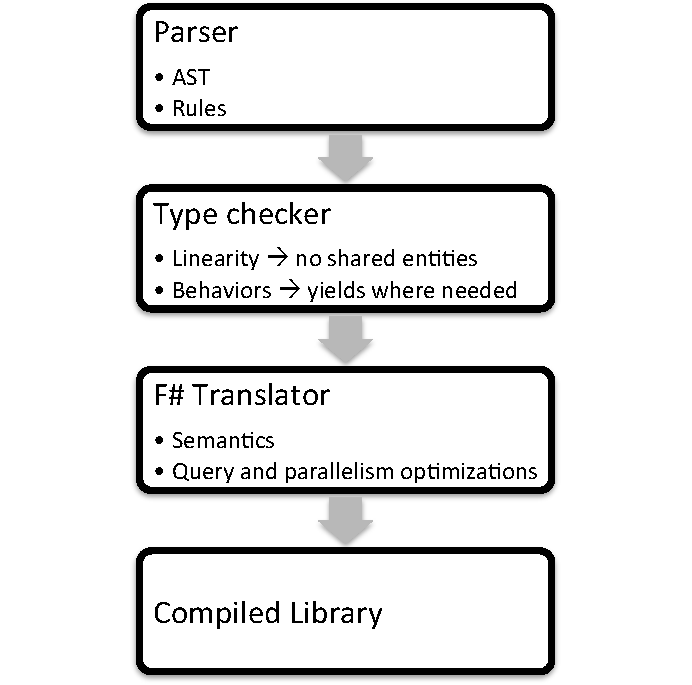
\includegraphics[scale=0.75]{compilation_process.pdf}
\end{center}
\caption{Compilation process}
\label{fig:compilation_process}
\end{figure}


\paragraph{Optimization}

Casanova performs three main optimizations.

The first optimization is a very simple one: memory recycling; even if simple, it can prove very effective in all those platforms (such as the Xbox 360) with a slow garbage collector. Memory recycling means that \texttt{Rule T} fields allocate a double buffer for storing both the $\mathtt{m}[r \rightarrow v]$ value and the $\mathtt{m}[r \Rightarrow v]$ value. Applying the $\oplus \mathtt{m}$ operator simply requires swapping the two buffers. The \texttt{Rule T} datatype is defined as:

\begin{lstlisting}
type Rule<'a> =
  {
    Values              : 'a[]
    FrameIndex          : int ref
  }
  member private this.ValueIndex
    with get() = this.FrameIndex.Value % this.NumValues
  member private this.ValueIndex' 
    with get() = (this.FrameIndex.Value + 1) % this.NumValues
  member this.Value
    with get() = this.Values.[this.ValueIndex]
    and set v' = this.Values.[this.ValueIndex] <- v'
  member this.Value'
    with get() = this.Values.[this.ValueIndex']
    and set v' = this.Values.[this.ValueIndex'] <- v'
\end{lstlisting}

all \texttt{Rule T}'s share the same reference to the current frame index. Whenever we wish to swap the references (that is when we apply the $\oplus$ function) then we just increment the \texttt{FrameIndex} without any need for traversing the entire state to manually set all \texttt{Rule T}'s.

This optimization can be extended to tables: at the beginning of each update, all values of type \texttt{Rule (Table T)} get their \texttt{Value'} cleared; clearing a table does not deallocate its elements: rather, it simply sets the counter of elements to zero, while keeping the previous memory allocated.

This strategy helps reducing the amount of garbage collection needed, sometimes giving large speedups as we can see in Section \ref{sec:benchmarks}.


The second optimization takes advantage of the static constraint that rules are linear: this means that no rules write the same memory location. We also know that rules may not freely write any references. These two facts guarantee thread safety, that is we may run or rules in parallel. Casanova dynamically allocates twice as many threads as the number of cores of the machine. Threads are only used to process lists of entities in the \texttt{GameState}, but no further multi-threading is performed: if an entity should contain many sub-entities those will all be processed sequentially in the same thread. This is needed to avoid creating too many threads; an excessive number of threads may even cause so much overhead that the benefits of parallelization are inferior to the losses in performance caused by the cost of threads.

The $i^{th}$ thread of $n$ will process the $i^{th}$ portion of each top-level table of the game state. This means that if the state is defined as:

\begin{lstlisting}
type GameState = 
  {
    Asteroids   : Table Asteroid
    Projectiles : Table Projectile
  }
\end{lstlisting}

then the $i^{th}$ thread will run the function:

\begin{lstlisting}
let thread state n i =
  for j = i * state.Asteroids.Count / n 
      to (i+1) * state.Asteroids.Count / n do
    update state.Asteroids.[j]
  for j = i * state.Projectiles.Count / n 
      to (i+1) * state.Projectiles.Count / n do
    update state.Projectiles.[j]
\end{lstlisting}

Unless the number of entities is very small or behaviors are very complex and computationally intensive, then the gains obtained by parallelization can be very high; the best results may even divide the duration of a tick by the number of threads, even if this is rarely the case.


The final optimization is query optimization. Nested list comprehensions (also known as ``joins'' in the field of databases) can have high computational costs; for example, the query:

\begin{lstlisting}
type Asteroid =
  {
    CollidingProjectiles 
      : Rule(Table(Foreign(Projectile)))
      :: \(state,self) -> [p | p <- state.Projectiles, collides(self,p)]     
  }
\end{lstlisting}

has a computational complexity of $O(n_p \times n_a) = O(n^2)$, where $n_p$ is the number of projectiles, $n_a$ is the number of asteroids and $n$ is the maximum between the two. Such a complexity is unacceptable when we start having a large number of asteroids and projectiles, because it may severely limit the maximum number of entities supported by the game.

We use the same physical optimization techniques used in modern databases: we build an index to speed up our collision detection. In particular, we observe that most asteroids and projectiles are so far away that testing them for collision does not make sense. We partition the space of the playing area into various blocks and we assign all our projectiles to the blocks they belong to; this operation costs $O(n_p)$ if blocks are a uniform grid and $O(n_p \log n_p)$ if blocks are of variable size and represented with a tree. For each asteroid, we find the blocks it belongs to ($O(n_a)$ or $O(n_a \log n_a)$) and then check for collisions only with the projectiles in those blocks. The final cost of the operation is $O(n)$ for hash maps and $O(n \log n)$ for trees.

An example hash map optimization could be the following. We add the following declaration to the game state:

\begin{lstlisting}
type GameState = 
  {
    ...
    Blocks   : Block[][]
  }
\end{lstlisting}

where a \texttt{Block} contains a list of projectiles.

In the update function we start by clearing the \texttt{Blocks} index and we fill it again with the updated projectiles:

\begin{lstlisting}
let update_state (state:GameState) (dt:float32) =
  for b in state.Blocks do
    b.Clear()
  
  for p in state.Projectiles do
    for b in p.Blocks do
      b.Add p
\end{lstlisting}

Benchmarks show that the costs of rebuilding the index are similar to modifying it, especially for trees. In this sense we confirm a similar result found in.

Collision detection will now become:

\begin{lstlisting}
let update_asteroid (state:GameState) 
                    (self:Asteroid) 
                    (dt:float32) =
  for b in self.Blocks do
    for p in b.Projectiles do
      if collides self p then
        self.CollidingProjectiles.Add p
\end{lstlisting}

A small bottleneck of this computation is the clearing phase, because it forces us to iterate all the blocks (which may be a large number for increased optimization) even if most of those are empty. For this reason, we further augment the state to track those blocks that contain projectiles (and thus which need clearing):

\begin{lstlisting}
type GameState = 
  {
    ...
    NonEmptyBlocks  : Table (BlockIndex)
  }
\end{lstlisting}

Now the update function becomes:

\begin{lstlisting}
let update_state (state:GameState) (dt:float32) =
  for bi in state.NonEmptyBlocks do
    state.Blocks.[bi].Clear()
  
  for p in state.Projectiles do
    for b in p.Blocks do
      b.Add p
      state.NonEmptyBlocks.Add b.Index
\end{lstlisting}

We must stress the importance of this last optimization. By having a function of quadratic complexity in the number of entities we are forcing our game to run with a maximum number of entities. Less entities often make for a less compelling game, because the world is less complex and the challenges are smaller. This class of optimizations allows the game performance to be less dependent on the number of entities. This means that we may design grander worlds with thousands of units and \textit{with no additional development complexity}.

\section{Case Studies}
\label{sec:case_study}
Mini Galaxy Wars.

\section{Benchmarks}
\label{sec:benchmarks}
%%%%%%%%%%%%%%%%%%%%%%%%%%%%%%%%%%%%%%%%%%%%%
% BENCHMARKS
%%%%%%%%%%%%%%%%%%%%%%%%%%%%%%%%%%%%%%%%%%%%%

- Windows, Xbox, Wp7 (, iPad?)
- memory recycling
- parallel execution
- query optimization


\bibliographystyle{plain}
\bibliography{references} 

\cite{*}
%\nocite{}

\end{document}
